\documentclass[a4paper,12pt]{article}
\usepackage[top=2cm, bottom=1.5cm, left=1cm, right=1cm]{geometry}
\usepackage{apacite}
\usepackage{amsmath}
\usepackage{graphicx}
\graphicspath{ {C:/Users/asus/Desktop/Latex} }

\begin{document}
\bibliographystyle{apacite}

\title{\textbf{{\large Fam Jiang Yuan, 1121116369}\vspace{5mm}\\Twitter as a Corpus for Sentiment Analysis and Opinion Mining}}
\author{\textbf{Alexander Pak, Patrick Paroubak}\vspace{5mm} \\Universit´e de Paris-Sud, Laboratoire LIMSI-CNRS, Bˆatiment 508,\\
F-91405 Orsay Cedex, France\\
alexpak@limsi.fr, pap@limsi.fr}
\date{}
\maketitle

\abstract{Microblogging nowadays became a most common communication tools for all Internet users. There are millions of users share their thoughts or opinions on different aspects of their daily life. Meanwhile, millions of corpus or even more, appear every day in popular social websites. Thus, microblogging websites are the idea platforms for opinion mining and sentiment analysis. In our research, we concentrate on one of the most popular microblogging website, Twitter, in order to perform sentiment analysis.  After that, we show how to collect a corpus from Twitter automatically and use it to train a sentiment classifier, which able to determine positive, negative, or neutral sentiment of a corpus. Throughout our experimental evaluations, we found that our methods are efficient and performs better than the previous existing methods. Besides that, we only worked on English, however, our proposed method can adapt on any language.}

\section*{\textbf{Problem Solved}}
In order to collect those corpus, we used a Twitter API to collect those valued information and then perform sentiment analysis by building a sentiment classifier, which able to determine positive, negative, or neutral sentiment for the collected corpus automatically.

\section*{\textbf{Claimed Contribution}}
First and foremost, we collect a corpus with positive and negative sentiment, and a corpus of objective texts by using our method that doesn't required human effort for classifying the collected corpus.
Next, we performed a statistical linguistic analysis of the collected corpus and used the collected corpus to train a sentiment classifier for microblogging.
Finally, we carried out an empirical evaluations by implementing the sentiment classifier on the real microblogging posts to prove that our methods are efficient and performs better than previous existing methods.

\section*{\textbf{Related Work}}
This research was referred to an existing work that presented by \cite{pang2008opinion}, who describe the existing methods and approaches for an opinion-oriented information retrieval. In \cite{yang2007emotion}, who used an emotion classifier to determine the sentiment level of the collected corpora by using Support Vector Machine (SVM) and Conditional Random Field (CRF) learning machine. J.Read \cite{read2005using}, who used emoticons to train the classifiers, which are SVM and Naïve Bayes, both classifier were able to obtain 70\% of accuracy during the test set. In \cite{go2009twitter}, authors used the similar approach, which using emoticons to get corpus sentiment on Twitter to collect the data and performed a sentiment analysis. So, the best obtained result goes to Naïve Bayes classifier as the classifier obtained 81\% of accuracy on the test set.

\section*{\textbf{Methodology}}
For corpus collection, we used a Twitter API and same approach as in (\cite{read2005using}; \cite{go2009twitter}) to collect a corpus of text posts and classify into positive sentiment, negative sentiment, and objective texts (no sentiment, neutral, or facts) with two types of emoticons, which are Happy emoticons and Sad emoticons. After that, those collected corpora were used to train a classifier to determine positive and negative sentiment of documents. We used English language in our research. 
For corpus analysis, we used a tool called TreeTagger \cite{schmid1994probabilistic} to tag all the posts in the collected corpora and then distribute the Part of Speech (POS)-tags. Moreover, we have compared the distributions of POS-tags and the results show that the positive texts are characterized by the positive ending, and the negative texts are characterized by the words of loss and disappointment.
For training the classifier, we used the existing of an n-gram as binary feature to extract the information. We have tested with unigrams, bigrams, and trigrams. Three of the n-gram perform differently at different aspects. Furthermore, we build a sentiment classifier by using the multinomial Naïve Bayes, since Naïve Bayes obtained the best results among SVM and CRF. Next, we have hand-annotated the outputs by testing our classifier on real Twitter posts. The results are presented in Table 1.

\begin{center}
\begin{tabular}{|l|r|}
\hline
Sentiment & Number of samples\\
\hline
\hline
Positive & 108\\
Negative & 75\\
Neutral & 33\\
Total & 216\\
\hline
\end{tabular}
\linebreak
\linebreak 
\textbf{Table 1}: The Characteristics of the evaluation dataset.
\end{center}

\begin{flushleft}
We evaluate the accuracy \cite{manning1999foundations} of our classifier using:
\end{flushleft}

\begin{equation}
accuracy = \frac{N(correct\:classifications)}{N(all\:classifications)}
\end{equation}

\begin{flushleft}
 We determine the accuracy across the classifier’s decision \cite{adda1998grace} using:
\end{flushleft} 

\begin{equation}
decision = \frac{N(retrieved\:documents)}{N(all\:documents)}
\end{equation}
\linebreak
\linebreak
The testing results are recorded and presented in graph.

\begin{center}
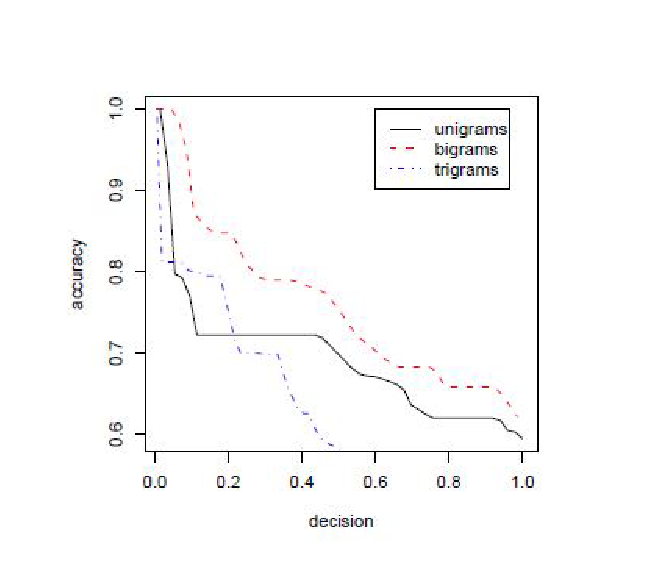
\includegraphics[scale=0.5]{graph.eps}
\linebreak
\linebreak
\textbf{Figure 1}: The comparision of the classification accuracy when using unigrams, bigrams, and trigrams.
\end{center}

\begin{center}
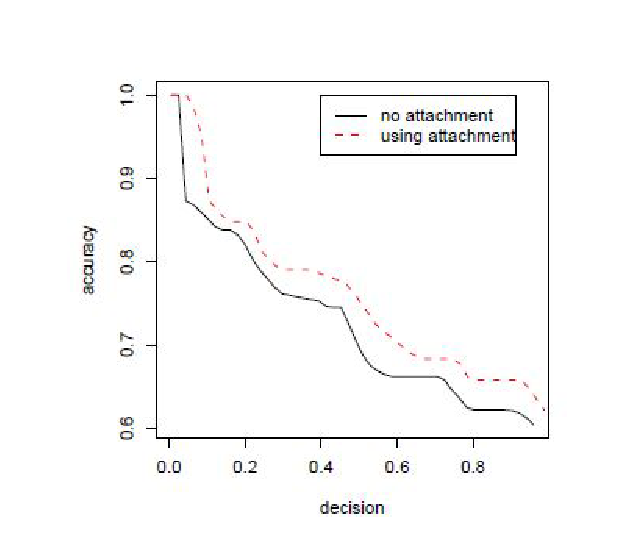
\includegraphics[scale=0.5]{graphs.eps}
\linebreak
\linebreak
\textbf{Figure 2}: The impact of using the attachment of negation words.
\end{center}

Throughout our testing results, we found that the best performance is obtained when using bigrams, as bigrams provide a balanced coverage (unigrams) and good ability to capture the sentiment expression patterns (trigrams).

\section*{\textbf{Conclusion}}
Microblogging nowadays became a most common communication tools for all Internet users. Microblogging websites is a platform where millions of corpus or even more, appear every day in popular social websites. Thus, microblogging websites are the idea platforms for opinion mining and sentiment analysis. In our research, we showed a method that can collect a corpus automatically and to be used to train a sentiment classifier. Next, we used Tree Tagger for POS-tag and observed the distribution among positive, negative, and neutral set. We trained a sentiment classifier known as Naïve Bayes that uses n-grams and POS-tags as features. Our trained classifier is capable to classify positive, negative, and neutral of document. 

\section*{Future Extension}
Throughout this research, I have learned some basic knowledge about data mining, and training a learning machine, in order to make the machine to make decision. However, the presented methodology in this research were limited in one language. So, as the future extension, the authors may plan to collect a multi-language corpus from microblogging websites and compare the collected corpora across with difference language to build a multi-language sentiment classifier.

\bibliography{mybib}
\bibliographystyle{plain}

\end{document}